\subsection{Análisis de tiempos en función de los parámetros de entrada}
En esta sección analizaremos de manera experimental como varían los tiempos de ejecución de los algoritmos descriptos al variar el largo y el ancho de la matriz y la cantidad de sanguijuelas del sistema.

\subsubsection{Ancho en función del tiempo}
Para comenzar, tomaremos un parabrisas con 50 sanguijuelas tal que estas solo afectan un punto de la discretización, y para una granularidad fija de $1.0$ iremos variando el largo del parabrisas. De esta manera, comenzaremos con un parabrisas de $50 \times 50$ luego uno de $60 \times 50$ y así aumentando de manera lineal ambos parámetros hasta llegar a un parabrisas de $100 \times 50$. Resolveremos cada uno de estos sistemas utilizando ambos métodos implementados (Gauss y Descomposición LU). Los resultados obtenidos pueden verse en el siguiente gráfico:

\begin{center}
 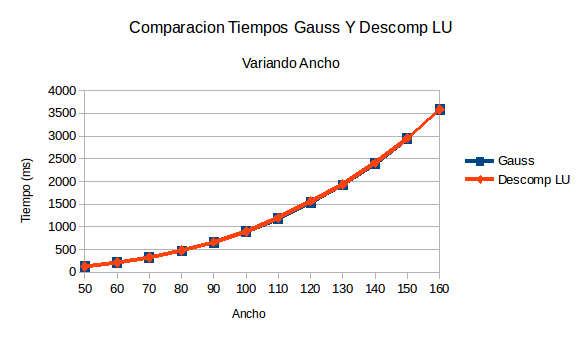
\includegraphics[width=400pt]{imagenes/testeo/anchoGauss.png}
\end{center}

Sabemos que al aumentar el largo del parabrisas de manera lineal, aumentará también de manera lineal el número de ecuaciones en nuestra matriz de resolución. Lo que puede observarse en este gráfico es que con un aumento lineal del largo del parabrisas, el tiempo de ejecución aumenta de manera semi-lineal. Esto era esperable ya que sabemos que tanto la Eliminación Gaussiana como la Descomposición LU tienen una complejidad igual a $O(n*p^2)$, y dado que en nuestro modelo utilizamos el largo del parabrisas para definir el tamaño de la banda en la matriz de resolución (es decir $p$), resulta lógico que al aumentar el largo, se obtuviera un aumento casi cuadrático en el tiempo de ejecución.
\\
Además, en este gráfico se pueden observar que tanto los tiempos de la factorización LU como la de Eliminación GAussiana son similares.
\\
Ahora, utilizando la misma familia de parabrisas descrita anteriormente, veremos cómo se comportan ambos métodos de salvación.
\\
Dado que nos aseguramos que cada sanguijuela solo toque un punto de la discretización, nos aseguramos que para cada una de las sanguijuelas podremos utilizar el método de Sherman-Morrison. Para estos algoritmos, el gráfico es el siguiente:
\\
\begin{center}
 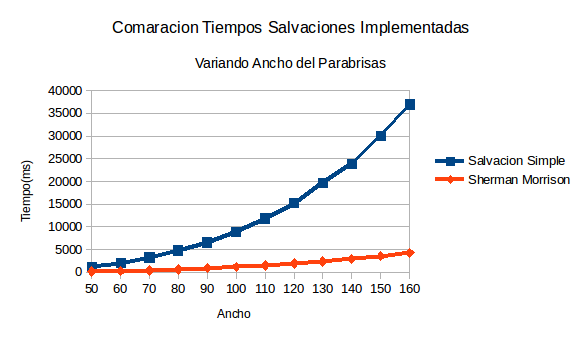
\includegraphics[width=400pt]{imagenes/testeo/anchoSalv.png}
\end{center}

Como era de esperar, el algoritmo que utiliza la optimización de Sherman-Morrison es mucho más rápido y escala mejor que la versión simple que debe calcular todo el sistema desde cero, ademas el Sherman-Morrison realiza operaciones sobre vectores y escalares haciendo la diferencia en el modo de comparación respecto al método anterior.

\subsubsection{Largo en función del tiempo}
Ahora analizaremos que sucede dejando fijo el ancho y variando el largo del parabrisas. Las condiciones son las mismas que en el test anterior, solo que ahora el ancho permanece constante igual a $50$ y se varía el largo de $50$ a $100$.

\begin{center}
 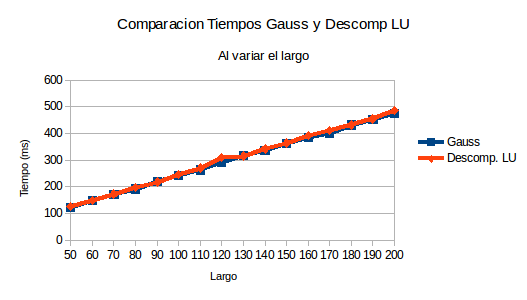
\includegraphics[width=400pt]{imagenes/testeo/largoGauss.png}
\end{center}

En este caso los tiempos de ejecución crecen de manera estrictamente lineal. Esto se debe que a diferencia del ancho, el largo no interviene en el cálculo del tamaño de la banda de la matriz de resolución. Luego, al aumentar el largo, solo aumenta la cantidad de incógnitas $n$.
\\
Aplicando el mismo experimento para los dos métodos de salvación:

\begin{center}
 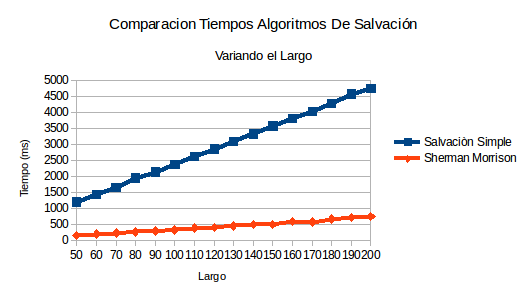
\includegraphics[width=400pt]{imagenes/testeo/largoSalv.png}
\end{center}

Al igual que lo dicho en la sección anterior, aquí también se pueden ver las ventajas de utilizar Sherman-Morrison. Además en este caso también puede apreciarse el comportamiento lineal de ambos algoritmos al variar el largo del sistema.

\subsubsection{Cantidad de sanguijuelas en función del tiempo}
Para el siguiente experimento, variamos la cantidad de sanguijuelas y dejamos fija tanto la granularidad como el largo y el ancho del parabrisas. Nuevamente, por una cuestión de simplicidad, las sanguijuelas solo afectan un punto de la discretización. Para el experimento tomamos un parabrisas de $100 \times 100$, una granularidad igual a $1.0$, y variamos la cantidad de sanguijuelas desde $10$ hasta $100$. Resolviendo el sistema con el algoritmo de Gauss y Descomposición LU, se obtuvo el siguiente grafico.

\begin{center}
 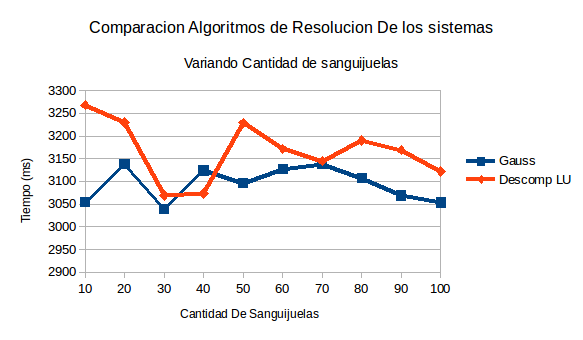
\includegraphics[width=400pt]{imagenes/testeo/sangGauss.png}
\end{center}

Como vemos, no se muestra ningún patrón visible al modificar la cantidad de sanguijuelas del sistema. Esto se debe a que la cantidad de incógnitas continúa siendo la misma.
\\
Ahora, utilizando el mismo experimento para el problema del último disparo, resolviendo este parabrisas con ambos algoritmos, se obtuvo este gráfico:

\begin{center}
 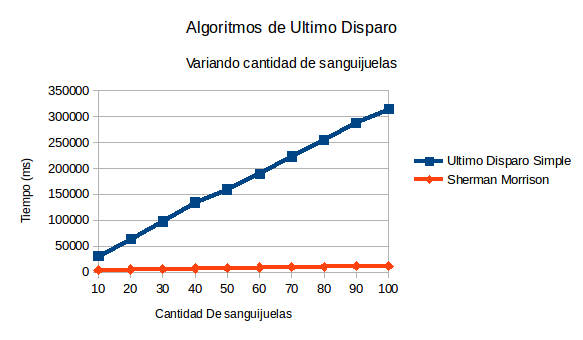
\includegraphics[width=400pt]{imagenes/testeo/sangSalv.png}
\end{center}

En este gráfico se puede apreciar cómo si bien ambos algoritmos dependen de manera lineal de la cantidad de sanguijuelas, el algoritmo de Sherman-Morrison presenta una mejor velocidad y una mejor escalabilidad.

\subsubsection{Granularidad en función del tiempo}
Por último, veremos como afecta variar la granularidad de la discretización para ver como se ve afectada la performance. Para este experimento se dejan fijos el largo y el ancho, iguales a $100$, la cantidad de sanguijuelas iguales a $5$ y se varía la granularidad desde $0.4$ hasta $0.9$, aumentando de $0.1$ en cada paso. Se obtiene lo siguiente:

\begin{center}
 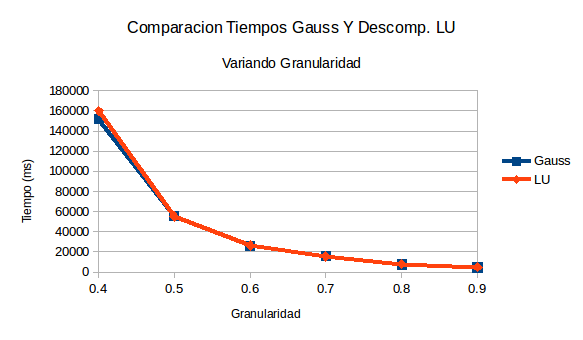
\includegraphics[width=400pt]{imagenes/testeo/granuGauss.png}
\end{center}

En el gráfico puede observarse que una disminución lineal de la granularidad produce un aumento cuadrático en el tiempo de ejecución. Esto se debe a que tanto la cantidad de filas y la cantidad de columnas viene dado por el largo/ancho del parabrisas, dividido por granularidad. Dado que el tamaño de nuestra matriz de resolución del problema viene dado por $\text{Cantidad De filas} \times \text{Cantidad De Columnas}$ esto será lo mismo que  $(\text{Largo} \times \text{Ancho}) / \text{granularidad}^2$. En esta fórmula puede verse claramente que disminuir la granularidad de manera lineal produce un aumento cuadrático en el número de incógnitas de nuestro problema.

\subsection{Análisis de temperatura en función de las discretizaciones}
El siguiente analisis que vamos a realizar sobre una instancia de 100 de largo por 100 de ancho con una sola sanguijuela en el punto $(45 45)$ de radio 1 con el fin de observar como afecta la granularidad al resultado del sistema y al punto crítico.
\\
Lo que esperamos observar es que para una granularidad mayor, el resultado posea un mayor grado de error, disminuyendo la precisión de la solución mientras que para granularidades menores el resultado se aproxime más al modelo continuo.
\\
Para ello tomamos 4 diferentes granularidades: $10, 5, 1$, y $0.5$.
\\
En el caso de una granularidad de $10$ la sanguijuela no podrá ser representada en ninguna de las ecuaciones del sistema, ya que no esta en contacto con ninguno de los puntos de la discretización. En este caso la respuesta arrojada por el algoritmo es la siguiente:
\begin{figure}[H]
\centering
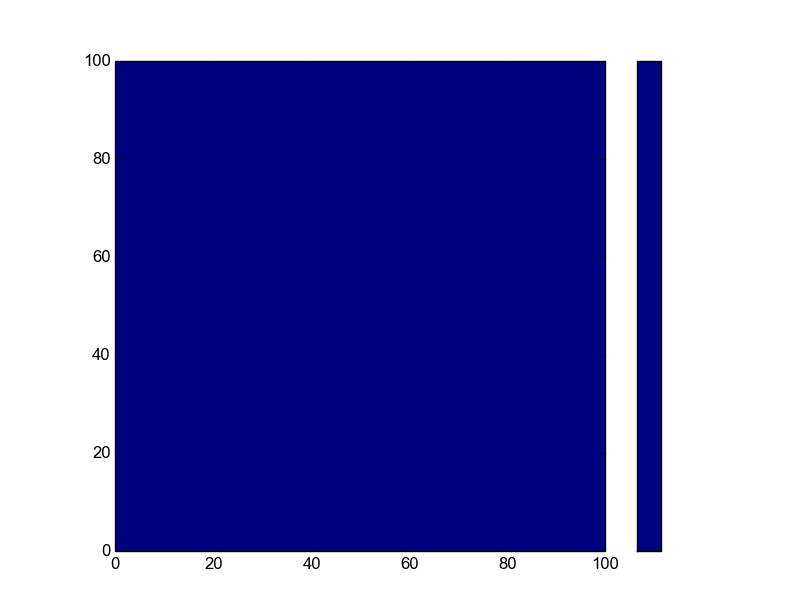
\includegraphics[width=400pt]{otrostests/11.png}    
\caption{ejecucion de 1sanguijuela10.in}
\end{figure}
Lo que intuitivamente sabemos es que no es correcto, ya que explícitamente agregamos una sanguijuela con una temperatura muy considerable. Sin embargo la temperatura del punto critico que el sistema calcula es de $-100$, por lo que uno esperaría encontrar en un sistema sin sanguijuelas.
\\
Para la granularidad de 5 ya es posible caracterizar a la sanguijuela en una de las ecuaciones, por lo que el gráfico obtenido será el siguiente:
\begin{figure}[H]
\centering

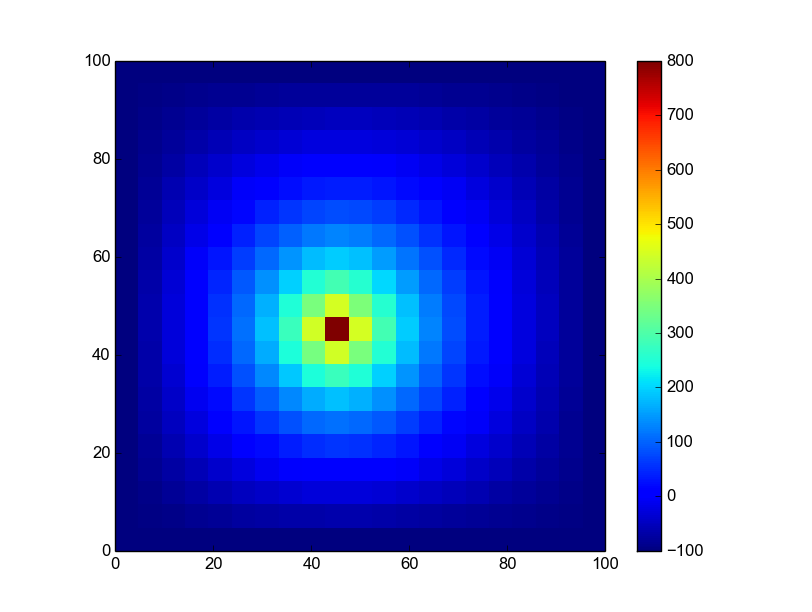
\includegraphics[width=400pt]{otrostests/12.png}
\caption{ejecución de 1sanguijuela5.in}

\end{figure}
\\
De esta manera podemos intuir que la respuesta es más próxima a la verdadera, ahora la temperatura del punto crítico es de $256.124$.
\\
Continuamos disminuyendo la granularidad, ahora con granularidad 1 se obtiene la siguiente respuesta:
\begin{figure}[H]
\centering

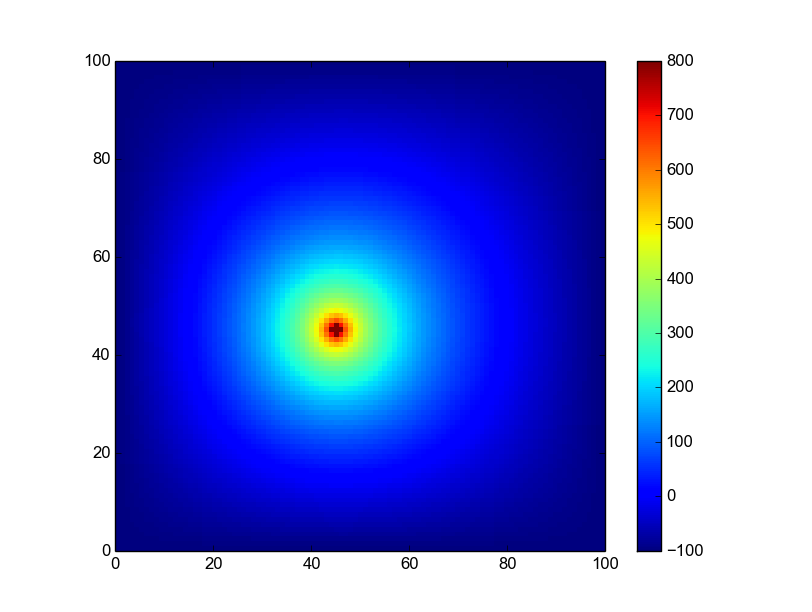
\includegraphics[width=400pt]{otrostests/13.png}
\caption{ejecución de 1sanguijuela1.in}

\end{figure}

Para esta respuesta ya pareciera que los resultados son más precisos, ya puede observarse cierta continuidad en la solución. Además otro hecho destacable es que la temperatura del punto crítico ahora es $333.008$, esto es un $30 \%$ mayor que para la granularidad anterior.
\\
Por último realizamos el mismo sistema pero para una granularidad de 0.1 obteniendo el siguente gráfico:

\begin{figure}[H]
\centering
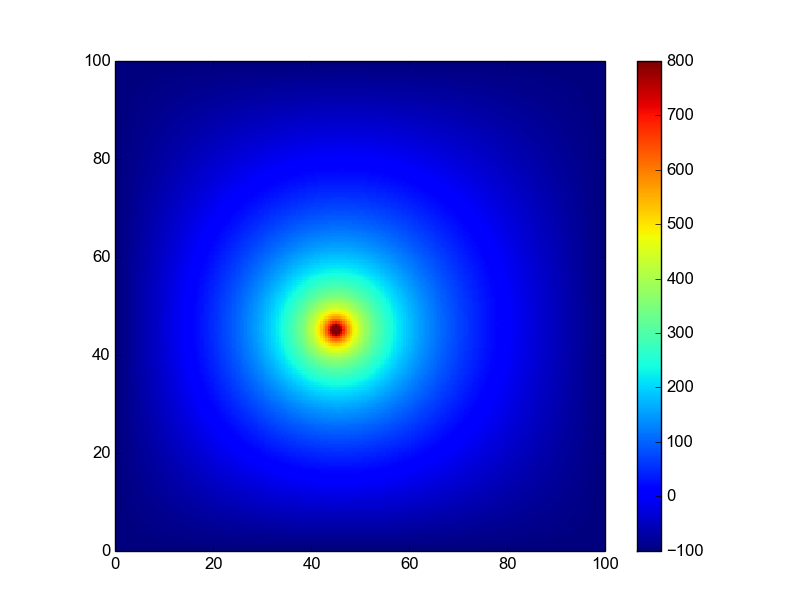
\includegraphics[width=400pt]{otrostests/14.png}
\caption{ejecución de 1sanguijuela0\_5.in}
 
\end{figure}

\\
Ahora ya es posible ver claramente la 'continuidad' de la solución. La temperatura del punto crítico es 335.65, osea un $0.7 \%$ mayor con respecto a la solución anterior.
\\
Puede notarse a simple vista que una granularidad más pequeña produce resultados que aproximan más exactamente a lo que uno creería es el resultado real de la ecuación diferencial de la que partimos en la introducción, ya que para una granularidad de $5$ pueden verse grandes bloques discretos, pero para la discretización de $0.1$ puede verse que estos bloques desaparecen y puede notarse una cierta 'suavidad' en el resultado obtenido, propio de una función continua y derivable. Esto puede verse en el gráfico ya que la tonalidad va oscureciendo hasta llegar a rojo generando un círculo grande, de ser chico estaríamos viendo un pico en la función y no sería derivable.
\\
Además, al disminuir la granularidad, está claro que la cantidad de incógnitas cercanas al punto crítico aumenta, por lo que, en caso de no poder tomarlo de manera exacta, al menos podremos tomar un vecino muy próximo a este por lo que tendemos a pensar que la presición del resultado también aumentará por ese lado.
Por último creamos 3 instancias del problema para ejecutarlas con dos granularidades distintas, uno y cuatro, para poder comparar mejor que pasaba con el punto crítico decidimos hacerlas de distintas medidas y sanguijuelas distribuidas de distinta forma para poder observar que ocurría.
Para el primer test, lo que se realizó fue una matriz cuadrada con 5 sanguijuelas las cuales estaban concentradas en la esquina izquierda inferior y otra en la esquina derecha superior, luego de correr Sherman-Morrison quitó la de la derecha superior que era la que tenía mayor temperatura y arrojó los siguientes gráficos de calor.

\begin{figure}[H]
 \centering
 \begin{subfigure}
  	
  	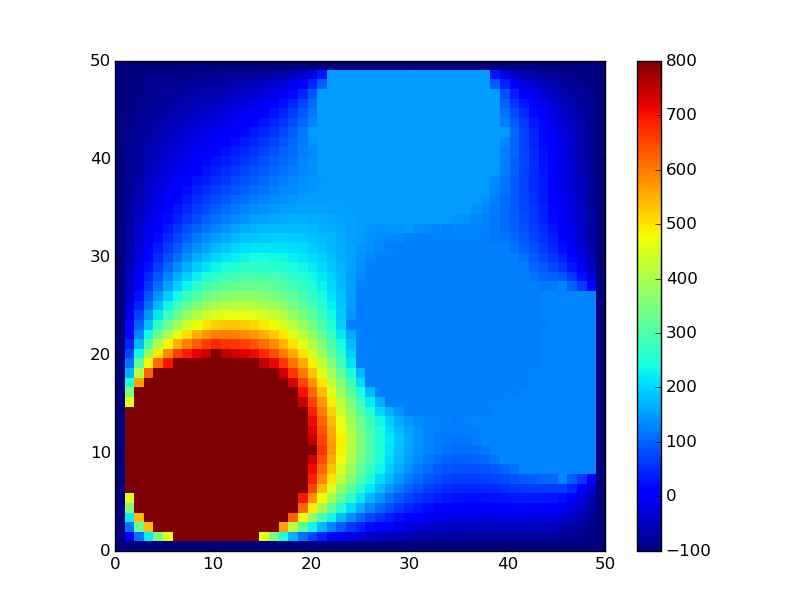
\includegraphics[width=300px]{imagenes/testpropios/test11.png}
  	\caption{ejecución test1.in}
 \end{subfigure}
 
 \begin{subfigure}
   	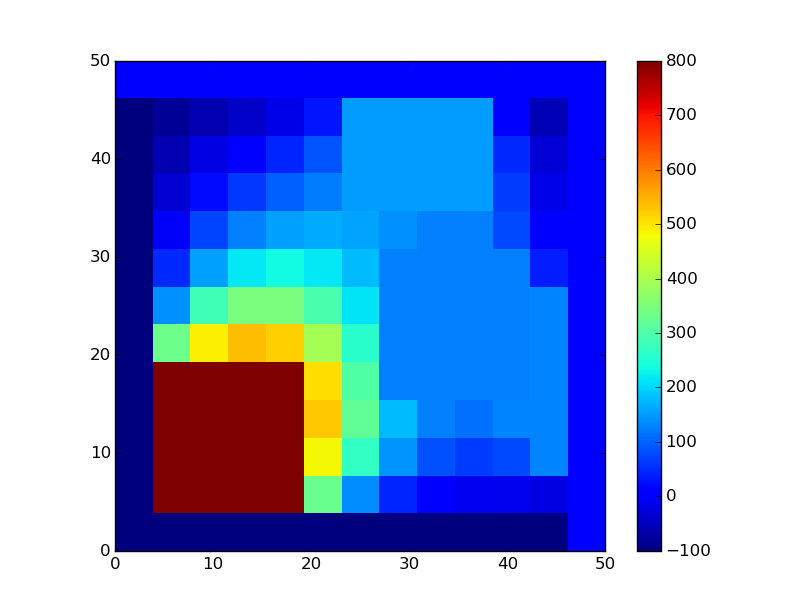
\includegraphics[width=300px]{imagenes/testpropios/test14.png}
    \caption{ejecución con granularidad 4, archivo test1b.in }
 \end{subfigure}
 
\end{figure}


Como se puede ver en este caso, y como mencionamos anteriormente a pesar de que las sanguijuelas estan en la esquina izquierda inferior el punto crítico se ve más afectado cuando la granularidad es mayor, dándonos en este caso una respuesta que no es correcta para el punto crítico ya que la imagen con menor granularidad en el punto crítico tiene menor temperatura, sabiendo que este último tiene menor precisión. 

Para el segundo se agranda el parabrisas y se agregan sanguijuelas, corremos el mismo test para los mismo valores de granularidad, uno y cuatro y obtuvimos el siguiente resultado.

\begin{figure}[H]
 \centering
   \begin{subfigure}
  		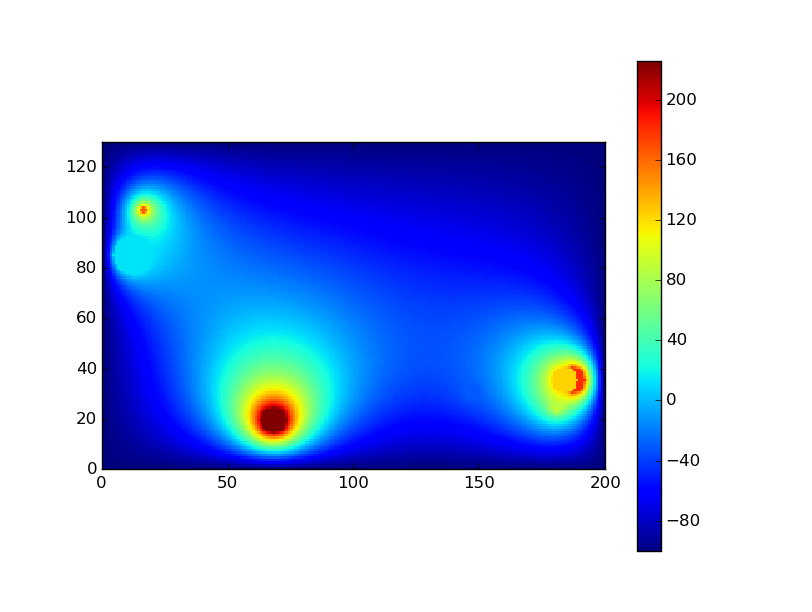
\includegraphics[width=300px]{imagenes/testpropios/test21.png}
    	\caption{ejecución test2.in}
   \end{subfigure}
  
   \begin{subfigure}
  		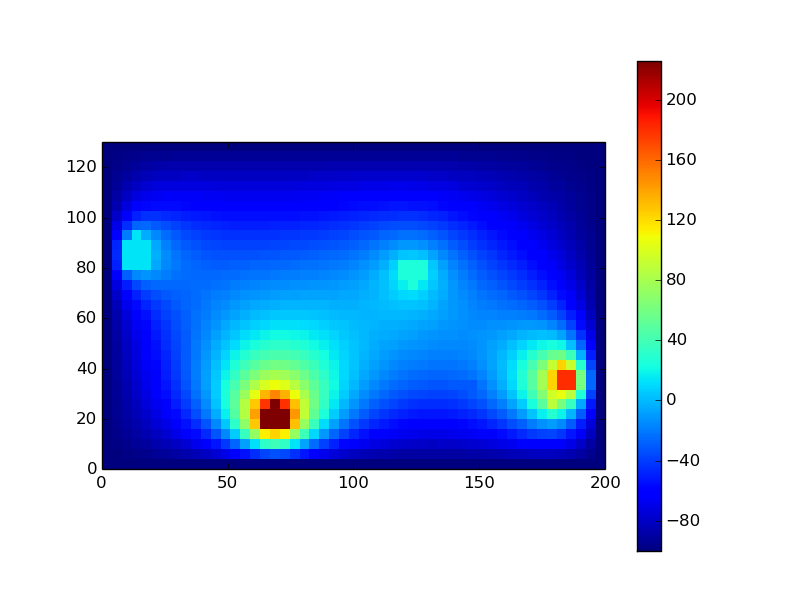
\includegraphics[width=300px]{imagenes/testpropios/test24.png}
    	\caption{ejecución test2b.in}
   \end{subfigure}

\end{figure}

A pesar que las sanguijuelas estan más repartidas volvemos a notar lo mismo que se veía en el primer test, a mayor granularidad mayor afectado se ve el punto crítico, a pesar que las sanguijuelas estan más alejadas.  

Por último alargamos más el parabrisas y corrimos el test para ver que era lo que sucedía, aunque como se comportaron los casos anteriores se espera que se repita el patrón, que cuanto mas granularidad más afectado se vea el punto crítico.
  \begin{figure}[H]
  \centering
 	\begin{subfigure}
  		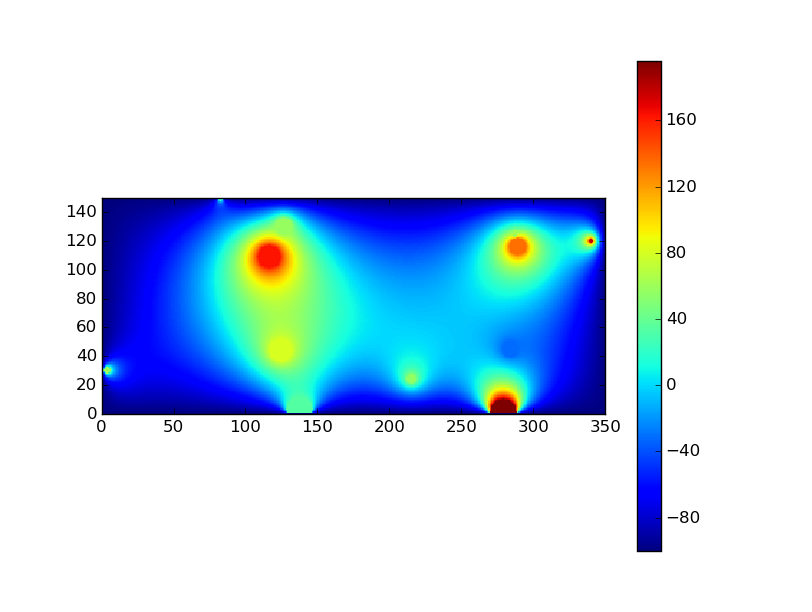
\includegraphics[width=300px]{imagenes/testpropios/test31.png}
    	\caption{ejecución test3.in}
	\end{subfigure}
	
 	\begin{subfigure}
 		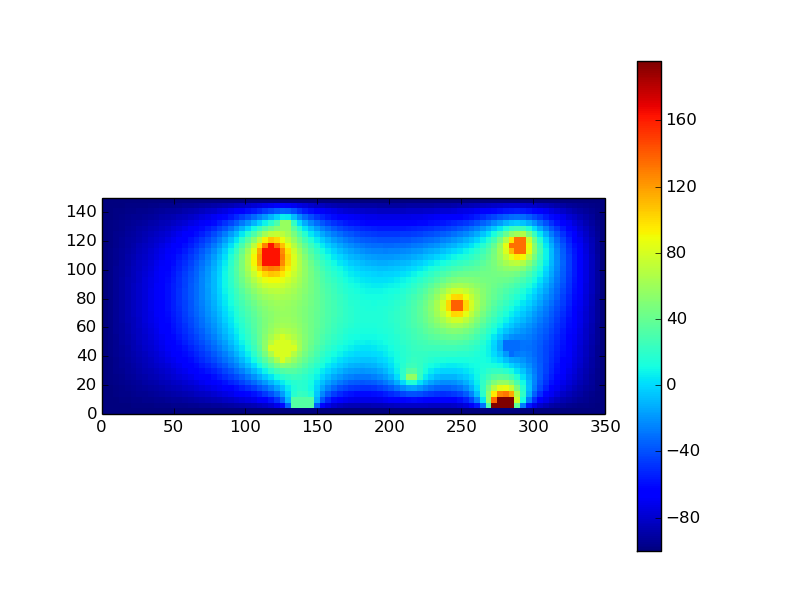
\includegraphics[width=300px]{imagenes/testpropios/test34.png}
    	\caption{ejecución test3b.in}
  \end{subfigure}

\end{figure}
Luego de realizar los tres test y notar que se repite el patron, de forma más particular en el ultimo caso ya que las sanguijuelas afectan las temperaturas haciendo que aumente la temperatura entre medio de ellas afectando el punto crítico.
Con lo cual podemos asegurar que mediante la granularidad sea más grande la precisión va a ser menor y el punto crítico va a ser mas afectados, y esto podria ser de suma importancia al momento de quitar la sanguijuela ya que podria afectar al punto critico al punto de remover otra sanguijuela porque su temperatura sobrepasa el límite.